\documentclass[10pt]{article}
\usepackage{a4wide}
\usepackage[english]{babel}
\usepackage{graphicx}
\usepackage{tabu}
\usepackage{textcomp}
\usepackage{fancyhdr}
\usepackage{lastpage}
\usepackage{titlesec}
\usepackage{lscape}
\usepackage{longtable}
\usepackage{color}
\usepackage{listings}
\usepackage{xkeyval}

\definecolor{mygreen}{rgb}{0,0.6,0}
\definecolor{mygray}{rgb}{0.5,0.5,0.5}
\definecolor{mymauve}{rgb}{0.58,0,0.82}

\lstset{ % Syntax highliughting for java
    backgroundcolor=\color{white},   % choose the background color; you must add \usepackage{color} or \usepackage{xcolor}
    basicstyle=\footnotesize,        % the size of the fonts that are used for the code
    breakatwhitespace=false,         % sets if automatic breaks should only happen at whitespace
    breaklines=true,                 % sets automatic line breaking
    captionpos=b,                    % sets the caption-position to bottom
    commentstyle=\color{mygreen},    % comment style
    deletekeywords={...},            % if you want to delete keywords from the given language
    escapeinside={\%*}{*)},          % if you want to add LaTeX within your code
    extendedchars=true,              % lets you use non-ASCII characters; for 8-bits encodings only, does not work with UTF-8
    frame=none,                    % adds a frame around the code
    keepspaces=true,                 % keeps spaces in text, useful for keeping indentation of code (possibly needs columns=flexible)
    keywordstyle=\color{blue},       % keyword style
    language=Octave,                 % the language of the code
    morekeywords={*,...},            % if you want to add more keywords to the set
    numbers=left,                    % where to put the line-numbers; possible values are (none, left, right)
    numbersep=5pt,                   % how far the line-numbers are from the code
    numberstyle=\tiny\color{mygray}, % the style that is used for the line-numbers
    rulecolor=\color{black},         % if not set, the frame-color may be changed on line-breaks within not-black text (e.g. comments (green here))
    showspaces=false,                % show spaces everywhere adding particular underscores; it overrides 'showstringspaces'
    showstringspaces=false,          % underline spaces within strings only
    showtabs=false,                  % show tabs within strings adding particular underscores
    stepnumber=5,                    % the step between two line-numbers. If it's 1, each line will be numbered
    stringstyle=\color{mymauve},     % string literal style
    tabsize=4,                       % sets default tabsize to 2 spaces
    title=\lstname                   % show the filename of files included with \lstinputlisting; also try caption instead of title
}
%%%%%%
%% Variables for version and release status
%% useage: \version
%%%%%%
\newcommand\module{CS25110}
\newcommand\moduleName{Internet And Systems Admin}
\newcommand\authorText{Nicholas Dart}
\newcommand\authorUsername{nid21}
\newcommand\studentID{130057750}
\newcommand\assesser{A.Shaw, S.Kingston, J.Gilbey}

%%%%%%
%% Alias
%%%%%%
\newcommand{\sectionbreak}{\clearpage}    %% Allways start a section on a new page


%%%%%%
%% Title and Author
%%%%%%
\title{ \huge \module Assignment \\ \Large \moduleName}
\author{
    \vspace{100pt}
    \begin{tabular}{ r || l }
        Author          & \authorText (\authorUsername)\\
                        & \studentID \\
        Date Published  & \today \\
                        & \\
        Assessed By     & \assesser \\
        Department      & Computer Science \\
        Address         & Aberystwyth University \\
                        & Penglais Campas \\
                        & Ceredigion \\
                        & SY23 3DB \\
    \end{tabular} \\
    %Copyright \textcopyright Aberystwyth University 2014
    %get rid of the date on the titlepage
    \date{}
}

\pagestyle{fancy}
\fancyhf{}
\lhead{\module~Assignment}
\rhead{\authorText~-~\studentID}
\rfoot{Page \thepage \hspace{1pt} of \pageref{LastPage}}
\lfoot{Aberystwyth University - Computer Science}

\begin{document}
    \maketitle
    {
        \centering
        \emph{Declaration of Originality}\\
    }
    In submitting this work, I confirm that: This submission is my own work, except where clearly indicated. I understand that there are severe penalties for plagiarism and other unfair practice, which can lead to loss of marks or even the withholding of a degree. I have read the sections on unfair practice in the Students’ Examinations Handbook and the relevant sections of the current Student Handbook of the Department of Computer Science. I understand and agree to abide by the University’s regulations governing these issues
    \thispagestyle{empty}
    \clearpage

    \tableofcontents
    \setcounter{page}{1}
    \clearpage

    \section{Introduction}
        The University of Coastal West Wales has been asked by the Welsh Government to allow small tech-based startups, local commerce and industry access to IT and infrastructure support as well as to provide working space for them. The newly appointed senior management team has also decided that, along side upgrading and adding infrastructure to support these startups and company's, the University's existing infrastructure for students and staff should also receive an upgrade as they are outdated by approximately five years.

        \subsection{Assumptions}
            \begin{itemize}
                \item The University currently provides some sort of visualized or \texttt{userdir} web hosting for students and staff
                \item The University currently provides file store facilities and a central server to staff and students to use
                \item The University currently has a total of 1000 work stations for staff and students
                \item The University currently has a Windows 7 Enterprise site license as well as a Microsoft Office site license
                \item The University currently uses some form of Active Directory service
                \item Each Business unit can contain at most 24 people
            \end{itemize}

    \section{Upgraded Web Services}
        \label{sec:webServices}
        This section covers upgrades or alterations to the University's web server infrastructure to support an additional 12 websites for use by startups, with details on how to expand this in the future. I am proposing two solutions, one for small to medium sites that do not receive large volumes of traffic, and can be easily scaled in the future with minimal cost, and a second solution for large sites that require high capacity and frequently have high loads. An ideal approach would be to use both solutions as needed, thus minimising maintenance and cost whist  maximizing quality of service for end users.
        
        \subsection{Virtual Hosts}
            Web servers can be set up to server multiple websites from the same physical machine, this is referred to as Virtual Hosts. Most main stream web servers (Eg apache, nginx, lighttpd) support either ip-based or name-based virtual hosts (herein referred to as \texttt{VHosts}), the former of which would be used here \cite{cite:apacheVHosts}\cite{cite:nginxServerBlocks}\cite{cite:lighttpdVHosts}. Virtual Hosts can be set up to allow multiple web sites to exist on the same physical server, running from the same instance of the web host. The University at present provides some sort of visualized web hosting for students, staff and departments, however for supporting commercial sites I recommend running them on a separate hardware dedicated for them. This way the University and Business services should not be effecting each other at busy or overloaded times. I also recommend buying at least one separate leased line to avoid overtaking the bandwidth capacity of the current University connection. 

            Depending on the traffic and load demands of the Business units, it may be possible to run 12 separate web servers on one physical machine, however for scalability and for quality of service, I would recommend a ratio somewhere between 2:1 and 4:1 virtual servers to physical machines.

            \subsubsection{Caveats}
                Virtual Hosts has the disadvantage that if the physical server goes down, it will take multiple websites offline. Similarly, if a single VHost is overloaded, other VHosts on the same physical machine will appear as if they are under heavy load. 

        \subsection{Dedicated Hosting with Leased Lines}
            This is a more conventional way of presenting web services, and is preferable for larger sized sites or sites with large traffic and bandwidth concerns. A dedicated leased line and dedicated web server for each site will allow for large volumes of traffic to each units web server and also allow them independence from each others faults and provide some protection from being overcapacity. 

            \subsubsection{Caveats}
                Whilst more suited for high-capacity sites, dedicated hardware and infrastructure will be more expensive initially and in running/maintenance. It will also prove difficult to scale in the future.

        \subsection{Additional Concerns}
            It is advisable to separate any resources not provided by the web server (external file store, \texttt{SQL} databases etc) on a separate machine not accessible from the outside/Internet. In both suggestions above, I have assumed this to be the case.

    \section{Computer Hardware}
        \label{sec:hardware}
        The University currently provides file storage, mail and logon services for student and staff. However these are out of date and need replacing. The new business units will also require new hardware, both for services provided by the university and machines for the new units they will be operating out of. It is understood that the new businesses operating out of these units may be mobile and as such will require hardware that is mobile. To this end I am making two recommendations for hardware for staff students and for the business units to accommodate different tasks.

        In my report blow, prices and quantities have been left out of this section, except where quantity assumptions or alterations have been made, but a full cost and quantity breakdown have been included within the Summary section (\ref{sec:summary}). I have also included within my quantity estimates spare and replacement machines where appropriate.

        \subsection{University Services and Server Room Hardware}
            As the university supports a large body of academic and research work, I have opted for very high performance hardware that should be able to scale with the university.

            \subsubsection{Servers}
                Due to the multiple roles this server will have to maintain: data computation, mail servers etc. I am recommending the \texttt{IBM System x3950 X6}\cite{cite:ibmx3950x6}. This server is a very high performance data processing server, I am assuming that two of these would be required, one for academic and admit purposes such as email, visualized machines and internal web hosting. I am then also assuming that a research or R\&D duplicate will also be available, whose purpose would be exclusively for research and large data computation tasks.
                Is I will mention in section \ref{sec:operatingSystems}, it may be desirable for multiple operating systems; to that end I propose that either a third \texttt{IBM System x3950 x6} be purchased, or existing hardware be re-tasked to support virtual machines for students and academic work that either required software systems that can be duplicated consistently or that are bespoke or unique and non-common.

            \subsubsection{Storage, NAS and SAN options}
                The storage solution I have chosen is the \texttt{Cyberstore-436s-zfs}\cite{cite:nexenta-NAS-cyberstore}. It is a very high capacity storage machine that can be configured in a NAS or SAN setup. It has onboard RAID 0+1, with support for additional hardware raid controllers. I am assuming the University's current NAS/SAN/JBOD setup can be migrated to this, with some reuse of the existing discs, however I have also included a recommendation for server grade hard drives. The \texttt{Cyberstore-436s-zfs}. I have also included 4-hour emergency support an on-site disaster recovery package, which may be utilized. The full specs for this server are as follows: 

                \begin{itemize}
                    \item Broadberry High-Density 4U 36 Bay with 1400Watt Redundant Power Supply, 6Gb/s Backplane
                    \item X9DRE-LN4F 16 Dimm Slots, QUAD Intel Gigabit LAN, On Board Graphics, On Board SATA RAID 0,1, IPMI \& Remote KVM
                    \item E5-2620 V2 Intel Six-Core Xeon 2.1GHz 15MB Cache - 80 Watts
                    \item 4GB 1600MHz DDR3 ECC Reg w/Parity DIMM Dual Rank
                    \item 6x 32GB 1600MHz DDR3 ECC Reg w/Parity DIMM Dual Rank
                    \item 35x 6TB Enterprise Class SAS2 6Gb/s 7200RPM - 3.5" - Seagate CONSTELLATION
                    \item 800GB Intel SSD S3500 DataCentre SERIES 2.5IN SATA3 MLC
                    \item LSI Host Bus Adaptor 8i (Non RAID)
                    \item 4x QLogic QLE2562 Dual Port 8-Gbps Fibre Channel (FC) to PCI-E (x8) Host Bus Adaptor (HBA)
                    \item NexentaStor Silver Edition 16TB
                    \item On-Site Disaster Recovery Bundle
                    \item 4 Hours Phone Support
                    \item 4 Hour Response
                    \item 9-5 Technical Support for System Lifetime
                    \item 48 Hour Comprehensive System Testing Procedure
                    \item UK Country Kit \& Mains Cable
                \end{itemize}


        \subsection{Student and Staff Desktop Machines}
            For most tasks, I feel an i3 desktop machine should suffice, I have chosen the \texttt{OptiPlex 3020 Micro}\cite{cite:3020micro}. It is a compact machine that should provide suitable for most students tasks, and provide a deacent office workstation for staff. This option also comes with a screen included in the price and a one year factory warranty. I have assumed a surplus of 50 units to be sufficient to cover replacement parts and dead-on-arrival units.

        \subsection{Business Unit Hardware and Resources}
            \subsubsection{File Storage}
                For each business unit I am recommending a separate NAS machine, specifically the \texttt{Thecus N8810U-G}\cite{cite:thecusNas}. I would also recommend adding in a hardware RAID controller in either RAID 50 or RAID 60 configuration to provide some data security and protection against loss. I am recommending a separate physical machine as it allows a unit to work independently any other, and will also allow for a larger number of people to operate out of one business unit. It also has the side effect that they could be located within the unit themselves if the main server room is a large distance away, thus decreasing network latency and increasing throughput. 

                It is also suggested in the brief that a mobile solution should be made available for the business units; but also maintain the ability to work on resources from the business. Therefore I advice the use of \texttt{Microsoft Surface Pro 3}\cite{cite:surfacePro3}. It is a portable device that can be used with a dock and monitors in the office, but can be equipped with a keyboard for field work. 

            \subsubsection{Web hosting}
                As I mentioned in the Web Hosting section (\ref{sec:webServices}), depending on the demands of the business unit, may warrant the use of either a virtual host or dedicated server for web hosting. I believe I have found a server that can support both tasks; the \texttt{PowerEdge R720 rack server}\cite{cite:dellPowerEdge} is a relatively powerful machine that should be able to support multiple virtual hosts, but also has support for a dedicated NIC card (Network Interface Card), and has the option to support plenty of storage should the business unit require it. I am assuming that to begin with, all the business units will be running off virtual hosts and so have only allocated 7 of these machines (6 for the units, and one as a redundancy should either a dedicated solution be required promptly, or in the event of failure of another)

            \subsubsection{Desktop Work Stations}
                I am making the assumption there will be a mixture (roughly a 50-50 split) between regular office users and `power users'; those who are doing computationally demanding tasks such as compiling software, video or image editing etc. To this end I am making recommendations of the following work stations.

                The \texttt{Dell Precision Tower 5810 Workstation}\cite{cite:powerWorkStation} for high end users. This can be ideal for a number of applications, and can support multiple graphics cards, a generous amount of ram (128gb), a variety of graphics and sound cards and several bays for Hard Drives.

                For the rest of the employees working in the business units, I recommend providing the \texttt{CyberStation 1150 Enhanced Office Workstation}\cite{cite:cyberstation}. It is suitable machine for almost all office tasks and should provide a good every day working machine for the employees. It can support a range of processor sockets, but I expect either the Intel i3 or i5 processors should be sufficient. 

    \section{Computer Software}
        \subsection{Operating Systems}
            \label{sec:operatingSystems}
            All machines in the hardware section above come pre-installed or have their operating system customized at purchase. The desktop machines I suggested under the hardware section come pre installed with Windows 7 Professional, This should be sufficient for most users however the University already has a site wide license for WIndows 7 Enterprise which can be used. It would also be likely for some desktop systems to require other operating systems such as Mac and Linux.

            I would recommend that any servers within the University use a Linux or Unix based Operating system such as Debian or FreeBSD unless a specific task requires otherwise. NIS.
        NIS.
        \subsection{Office software}
            As the University already has a software license for Microsoft Office, unless that requires updating I am assuming that the current version is suitable for use. I would also recommend a software package that supports OpenOffice standards such as Libre Office be installed on all university computers for students that do not have or use Microsoft products. Other bespoke software such as Image editing, software development etc. software will most likely be required by departments throughout the university, but I am assuming that will be either already available or purchased as needed. 

        \subsection{Enterprise or Business Software}
            The business units will most likely require or expectNIS.NIS. certain software to be installed suck as Microsoft Office, Outlook etc. Other software tools such as Microsoft Project or TeamFoundation Server will probably be required for time management facilities. Beyond that I suggest that software is purchased on an as-needed basis. 

            For web hosting I also recommend using one of the web servers I mentioned in Upgrading Web Services section; Apache, nginx or lighttpd. Apache is the most common web server and has the most support, however nginx is better for large sites with many concurrent connections, but with the penalty of reduced support for modules and no official support unless a license is purchased. Lighttpd is the third option I am suggesting, it is a very light weight and fast asynchronous web server designed for scalability of limited hardware\cite{cite:lighttpdWiki}.

            For the task of the business units, I am inclined to not offer a single opinion; however for large scales I am more inclined towards nginx

        \subsection{Miscellaneous Software}
            As the University provides educational courses, It has other bespoke software it will require either licences for, or permission to use. I am assuming any such licences are site-wide and do not need re-purchasing. 

    \section{Security}
        The University is required by law to adhere to the Data Protection Act 1998\cite{cite:dataProtectionAct}, to aid with this, I propose the following overarching security desires:

        \begin{enumerate}
            \item To prevent theft, loss or corruption of data or IP
            \item To prevent loss of physical hardware
            \item To prevent service downtime, unauthorized or malicious use
        \end{enumerate}

        I recommend the University follows the ISO standard 17799:2005 - Information technology and Security techniques\cite{cite:iso17799:2005}, this sets forth guidelines for setup, maintenance and upgrade to information security in a general non-medium specific way that can be applied across the university and applies to data storage and protection for the business units.

        To address the concerns of physical security, I suggest an inventory of all hardware be kept and maintained with serial numbers and identifiable information. I would also suggest that the ability to remove such hardware from the premises be minimized as much as possible through the use of security locks and tethers or cages. For more sensitive areas such as data stores or high value servers and services that entrance be restricted to authorized, knowledgeable personnel. Any entry to these areas should be monitored and logged and these log should be reviewed. Staff should also be trained to report entries on unknown personnel to these areas to relevant people or departments. Any person requiring entry to secured areas who is not permitted should require approval from the department(s) who administer and maintain the hardware in these areas and should be monitored at all times. 

        Security concerns for data and intellectual property can be mitigated through the use of separate networks where possible for sensitive data, and where this is not practical, limiting the access to the bare minimum. Security critical data should also be protected using some form of encryption. Any data who's content does not need to be know, but needs to be compared such as passwords should not be stored using reversible encryption, and instead hashed.

        As a data controller, the university is required to keep the data no longer than is required for it's purpose, and similarly must use the data solely for the reasons specified under it's contract with the data provider. It is, however, the responsibility of the data provider to keep the data they provide up to date and correct. 

    \section{Naming and Directory Services}
        DNS is the primary and most commonly used naming service use for IP resolution, and is supported by almost all hardware. However DNS as a sole solution would be impractical. DNS does not provide a collective database of resources such as printers, storage, user databases etc. Therefore the use of services such as \texttt{LDAP} would be advisable\cite{cite:ldap}. Services such as \texttt{BIND}, which are the most commonly used services for DNS resolution, can be used, and most likely are already in use within the university\cite{cite:bind}.

        As for directory services, I recommend using \texttt{samba} on the filestore. \texttt{samba} is a GNU open source implementation of the Microsoft Active Directory Services. It allows files to appear as if they are directly connected to a machine whist actually being stored on a server, NAS or SAN elsewhere on the network. It can provide seamless mounting of users directories on logon to machines throughout campus and the business units. 

    \section{Project Management}
        The proposed task of upgrading the universities infrastructure is a large, long and expensive undertaking, the traditional model of development for projects such as are the waterfall method, I believe this to be a bad method of development as it reduces communication and responsiveness to changes in circumstances. Whilst it does provide clear focus on the end goal and there are very clear goals and deliverables that need to be met. I recommend instead a model of management and development that reduces risk and attempts to disclose obstacles and unforeseen challenges early in the project, such as the spiral model. This approach starts with concepts and works it's way up to progressively larger phases of implementation and action, with each phase more certain of how tasks and goals should be tackled. I feel the main goals of each iteration of the spiral should be the following:

        \begin{enumerate}
            \item Iteration 1:
                \begin{enumerate}
                    \item Understand the main goals and hazards of upgrading the infrastructure of the university
                    \item Understand what is required by a business unit, what resources are present and what are now
                    \item Find, understand and research requirements for existing business units
                \end{enumerate}
            \item Iteration 2:
                \begin{enumerate}
                    \item Find local businesses and collaborate to understand their requirements and desires/future plans
                    \item Ask student body, departments and staff for desired outcomes of the university infrastructure upgrade
                    \item Research feedback from businesses and the wider university
                \end{enumerate}
            \item Iteration 3:
                \begin{enumerate}
                    \item Planning for upgrades and construction of infrastructure for business units
                \end{enumerate}
            \item Successive Iterations:
                \begin{enumerate}
                    \item Implementation of plan, iterations with and feedback from the businesses and wider university
                \end{enumerate}
        \end{enumerate}

        In addition to the spiral method, it is advisable to keep or if possible expand communication between departments, the IT upgrade/management team and existing users of the system; an approach such as agile would suffice. This way the entire department should be knowlidgable of the desired events and possible problems of the days work, and can keep other parts of the university informed\\
        {
            \centering
            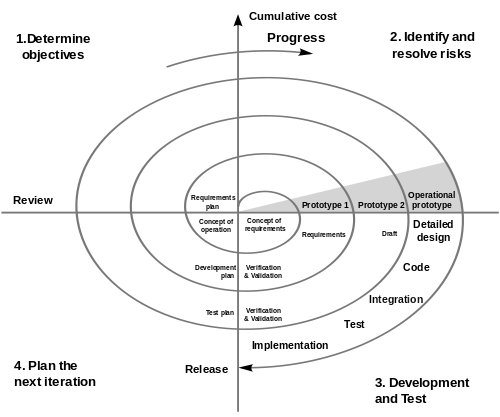
\includegraphics[scale=0.75]{spiralmodel.png}
        }

    \section{Business Continuity}
        Steps and plans should be prepared ahead of time for emergency scenarios such as fire, theft or loss of data. In particular staff managing high priority or business critical data need to be trained how to react and what tasks need to be performed in the event of these emergencies.

        Precautions should also be taken during planning and execution of the upgrade phase to the university. It should be carried out at a time of minimal activity and try to provide a seamless transition. To this end I recommend ordering parts and hardware early and if possible, dry running instillation and setup tasks before hand. Spare parts and redundancies should also be accounted for when an upgrade of this scale is undertaken. 

        \subsection{Risk Analysis}
            Whilst it is not possible to be prepared for the unforeseeable, specific and general risk analysis should be performed for eventualities such as fire, water damage, hardware failure, data loss or theft, staff loss or service outages. Responses to these scenarios should be planned, with temporary work-around sand steps to recover from them. 

        \subsection{Backups}
            Backups are critical to continued operation of both the university, and the business units. Short term backups should be taken at intervals relevant to the data and how often it changes. It is advisable to take cascaded backups where possible; nightly backups, then once a week a backup of the most recent data is taken.
            Off site backups should also be taken to ensure natural disasters and other unforeseen accidents do not destroy data stored in the same physical location. These should also have some form of data protection to prevent theft.

        \subsection{Redundancy}
            As I have used repeatedly in the Hardware section (\ref{sec:hardware}), RAID is an easy way of making data at least semi-redundant. However it is not a complete backup solution, as redundant data can still be lost if multiple discs in the RAID array fail without being replaced and allowed to be rebuilt. 


    \section{Ongoing Management}
        As the initial brief said, the university is to take on 12 business units, potentially more to follow. Whist I have tried to encompass future expansion of both the university and these units, eventually this process will need to be repeated. I therefore suggest regular reviews of the usage of resources and the wear-and-tear of devices and hardware. 

        \subsection{Future Technologies to consider}
            This section is purely my opinion of future technological advances and ones that may prove noteworthy to invents in.
            \\
            Fibreoptics; whist the University most likely already uses fibre optics for it's external ADSL lines and inter-building communications, I feel it's worth reiterating that it is a technology that can be upgraded relatively easily. Short distance communications can be improved by replacing the fibre optics cards at either end. 

            Thunderbold and USB type c and display port; higher throughput IO will probably become more common place. As the information revolution continues, we will be transferring more and more data around with us.

            Encryption and security, in the wake of the Snowden leaks, is a more important issue than ever. How the university stores and manipulates data will be of an ever increasing concern for users. 

    \section{Summary}
        \label{sec:summary}
        \subsection{Price Summary}
            \begin{tabular}{| p{8cm} | r | r | r |}
                \hline
                    & Unit Price & Quantity & Total \\ \hline
                    Servers & & & \\ \hline
                    PowerEdge r720 & \textsterling1,300 & 7 & \textsterling9,100 \\ \hline
                    Thecus N8810UG & \textsterling1,800 & 12 & \textsterling21,600 \\ \hline
                    Cyberstore-436s-zfs & \textsterling32,000 & 4 & \textsterling136000 \\ \hline
                    IBM x3950x6 & \textsterling100,000 & 2 & \textsterling200,000 \\ \hline
                    & & & \\ \hline
                    Work Stations & & & \\ \hline
                    Dell Precision t5810 & \textsterling1,100 & 150 & \textsterling160,000 \\ \hline
                    CyberStation 1150 Enhanced Office Workstation & \textsterling300 & 150 & \textsterling45,000 \\ \hline
                    Surface Pro 3 & \textsterling670 & 144 & \textsterling92,000 \\ \hline
                    Optiplex 3020m & \textsterling420 & 1000 & \textsterling420,000 \\ \hline
                    & & & \\ \hline
                    Total & & & \textsterling1,224,000 \\ \hline
            \end{tabular}

            These prices are not including any bulk or educational discounts

    \clearpage
    \begin{thebibliography}{9}
        \bibitem{cite:apacheVHosts}
            http://httpd.apache.org/docs/2.2/vhosts/
        \bibitem{cite:nginxServerBlocks}
            http://wiki.nginx.org/ServerBlockExample
        \bibitem{cite:lighttpdVHosts}
            http://redmine.lighttpd.net/projects/1/wiki/docs\_modsimplevhost
        \bibitem{cite:lighttpdWiki}
            https://wiki.archlinux.org/index.php/lighttpd
        \bibitem{cite:dellPowerEdge}
            http://www.dell.com/us/business/p/poweredge-r720/fs
        \bibitem{cite:thecusNas}
            http://www.thecus.com/product.php?PROD\_ID=102
        \bibitem{cite:webHosts}
            http://news.netcraft.com/archives/2014/02/03/february-2014-web-server-survey.html
        \bibitem{cite:dataProtectionAct}
            http://www.legislation.gov.uk/ukpga/1998/29/contents
        \bibitem{cite:iso17799:2005}
            http://www.iso.org/iso/iso\_catalogue/catalogue\_ics/catalogue\_detail\_ics.htm?csnumber=39612
        \bibitem{cite:powerWorkStation}
            http://www.dell.com/uk/business/p/precision-t5810-workstation/pd
        \bibitem{cite:cyberstation}
            http://www.broadberry.co.uk/intel-core-i5-workstations/cyberstation-i5-enhanced-office
        \bibitem{cite:nexenta-NAS-cyberstore}
            http://www.broadberry.co.uk/nexenta-storage-servers/cyberstore-436s-zfs
        \bibitem{cite:ibmx3950x6}
            http://www-03.ibm.com/systems/uk/x/hardware/enterprise/x3950x6/index.html
        \bibitem{cite:3020micro}
            http://www.dell.com/uk/business/p/optiplex-3020m-desktop/pd?oc=ca005d3020m11\&model\_id=optiplex-3020m-desktop
        \bibitem{cite:bind}
            http://www.isc.org/downloads/bind/
        \bibitem{cite:ldap}
            http://www.openldap.org/
        \bibitem{cite:surfacePro3}
            http://www.microsoft.com/surface/en-gb/products/surface-pro-3
    \end{thebibliography}

\end{document}